\section{B\"{u}chi Automata}
We now know if a path of an FTS satisfies a given LTL formula, however we are interested in \textit{generating} paths that satisfy a given formula, which requires a significantly more amout of work! We are going to need a finite representation of a given LTL formula, that we can search. This representation is a Nondeterministic B\"{u}chi automaton (NBA). 
\begin{definition}
\label{defNBA}
An NBA $\mathcal{A}_\varphi$ is defined by a five-tuple:
\begin{align*}
\mathcal{A}_\varphi = (\mathcal{Q},2^AP,\delta,\mathcal{Q}_0,\mathcal{F})
\end{align*}
where $\Q$ is a finite set of states, $\Q_0 \subseteq \Q$ is the set of initial states, $2^{AP}$ is the alphabet, $\delta: \Q \times 2^{AP} \rightarrow 2^\Q$ is a transition relation, and $\mathcal{F} \subseteq \Q$ is the set of accepting states
\end{definition} 
An infinite run of an NBA is an infinite sequence or states, $r=q_0 q_1 \dots$, where that starts from an initial state i.e.\ $q_0 \in Q_0$ and $q_{k+1} \in \delta(q_k, S)$ for some $S \in 2^{AP}$, for $k = 0,1,\dots$. The requirements for a run $r$ to be accepting is $\Inf(r) \cap \F \neq \emptyset$, where $\Inf(r)$ is the set of states that appear in $r$ infinitely often \cite{guo15}. 

Now to tie together the concept of words and runs on an NBA. An infinite word $\sigma = S_0 S_1 \dots$ corresponds to $r_\sigma = q_0 q_1 \dots$ where $q_0 \in Q_0$ and $q_i+1 \in \delta(q_i,S_i)$

It has been shown that given an LTL formula $\varphi$ over $AP$, there exists a NBA over $2^{AP}$ corresponding to $\varphi$, denoted $A_\varphi$ \cite{baier08}. When we say an NBA corresponds to an LTL formula, we mean that the set of words that correspond to accepting runs of the NBA is the same as the set of words accepted by the LTL formula.  

\section{Product Automata}
These two structures are then combined to create the product automaton. The product automata is also a B\"{u}chi automata and is defined as follows:
\begin{definition}
The weighted product B\"{u}chi automaton is defined by $\mathcal{A}_p = \mathcal{T} \otimes \mathcal{A}_\varphi = (Q', \delta', Q_0', \mathcal{F}', W_p)$, where $Q' = \Pi \times Q = \{ \langle \pi, q \rangle \in Q' | \forall \pi \in \Pi, \hspace{0.2cm} \forall q \in Q \}$; $\delta: Q' \rightarrow 2^{Q'}$. $\langle \pi_j, q_n \rangle \in \delta' (\langle \pi_i, q_m \rangle )$ iff $(\pi_i , \pi_j ) \in \rightarrow_c$ and $q_n \in \delta (q_m, L_c(pi))$; $Q_0' = \{ \langle \pi , q \rangle | \pi \in \Pi_0, \hspace{0.2cm} q_0 \in Q_0\}$, the set of initial states: $\mathcal{F}' = \{ \langle \pi, q \rangle | \pi \in \Pi, q \in \mathcal{F}$, the set of accepting states; $W_p: Q' \times Q' \rightarrow \R^+$ is the weight function: $W_p(\langle \pi_i, q_m \rangle , \langle \pi_j, q_n \rangle ) = W_c (\pi_i, \pi_j)$, where $\langle \pi_j, q_n \rangle \in \delta' ( \langle \pi_i, q_m \rangle )$
\end{definition} 

Given a state q' = $\langle \pi, q \rangle \in Q'$, its projection on $\Pi$ is denoted by $q'|_\Pi = \pi$ and its projection on $Q$ is denoted by $q'|_Q = q$. Given an infinite run $R = q_0' q_1' a_2' \dots$ of $\mathcal{A}_p$, its projection on $\Pi$ is denoted by $R|_\Pi = q_0'|_\Pi q_1'|_\Pi q_2'|_\Pi \dots$ and its projection on $Q$ is denoted by $R|_Q  = q_0'|_Q q_1'|_Q q_2'|_Q \dots$ \cite{guo15}. 

Given that $\A_p$ is a B\"{u}chi automaton, the requirements of an accepting run, r, is the same as before i.e.\ $\Inf(r) \cap \F \neq \emptyset$

\begin{lemma}
If there exists an infinite path $\tau$ of $\T_c$ such that $\tau \models \varphi$, then at least one accepting run of $\A_p$ exists.
\end{lemma}
Proof. see the proof of Theorem from [11] meng

\begin{lemma}
\label{lemma1}
If $R$ is an accepting run of $\A_p$, then $R|_\Pi \models \varphi$ 
\end{lemma}
Proof. see proof in meng

Given \ref{lemma1}, our problem is now to find an accepting run of $\A_p$. Given that an accepting run is a infinite sequence of states, and there are infinitely many possibilities, the process of finding one, nonetheless finding one that has measure of optimality is non-trivial, both theoretically and practically meng "both in theory and software implementation". Therefore we restrict our view of accepting runs to runs that satisfy the prefix-suffix structure i.e.\
\begin{align*}
\tau = \langle \tau_{pre}, \tau_{suf} \rangle = \tau_{pre} [\tau_{suf}]^\omega
\end{align*}
The prefix, $\tau_{pre}$, in our case is going to be a path from an initial node to an accepting node. The suffix, $\tau_{suf}$, is going going to be a path from the same accepting node back to itself. So the full path is going to be the prefix and then the suffix repeated infinitely many times (which is the meaning of the $\omega$ superscript). Thus, the accepting node appears infinitely many times in $\tau$ which makes $\tau$ accepting. Plans of this form are much easier to deal with because, while they are still infinite plans, they have a finite representation that we can exploit.

\section{Cost of a Run}
We are focusing on the accepting runs of $\A_p$ with the prefix-suffix structure
\begin{align*}
R &= \langle R_{pre}, R_{suf} \rangle = q_0 q_1 \dots q_f [q_f q_{f+1} \dots q_n]^\omega \\
&= \langle \pi_0, q_0 \rangle \dots \langle \pi_{f-1}, q_{f-1} \rangle [ \langle \pi_f , q_f \rangle \langle \pi_f , q_f \rangle \dots \langle \pi_{n}, q_n \rangle ]^\omega
\end{align*} 
from meng
where $q_0 = \langle \pi_0, q_0 \rangle \in \Q_0$ and $q_f = \langle \pi_f , q_f \rangle \in \F$. There is a finite set of transitions in our infinite path i.e.\ 
\begin{align*}
\Edge (R) = \{(q_i, q_{i+1}) , i = 0,1,\dots ,(n-1)\} \cup \{(q_n , q_f ) \}.
\end{align*}
Each of these transitions has a cost, given by $W_p(q_i,q_{i+1})$ allowing us to define the total cost of $R$ as
\begin{align*}
\Cost (R, \A_p) &= \sum_{i=0}^{f-1} W_p(q_i,q_{i+1}) + \gamma \sum_{i=f}^{n-1} W_p(q_i,q_{i+1}) \\
&= \sum_{i=0}^{f-1} W_c(\pi_i,\pi_{i+1}) + \gamma \sum_{i=f}^{n-1} W_c(\pi_i, \pi_{i+1})
\end{align*}
where $\gamma \geq 0$ is the relative weighting of the transient response (prefix) cost and steady response (suffix) cost. We then look for the accepting run with prefix-suffix structure that minimizes the total cost. 

We will denote this accepting run as $R_{opt}$, with the corresponding plan $\tau_{opt} = R_{opt}|_\Pi$. We note however that this plan may not actually be the true optimal plan with prefix-suffix structure. In \cite{schuppan05} we see that simplifications in the translation from LTL formulas to NBA can result in a loss of optimality. This will be important when we analyse the paths our algorithm generates. 

\section{Search Algorithm}
The search algorithm used in many recent works on the specific type of control planning synthesis comes from this prefix-suffix structure. The basic idea is to find a path from an initial node, $q_0$ to an accepting node, $q_f$, and then find a path from the $q_f$ back to itself. The first part from $q_0$ to $q_f$ is the prefix and the second part $q_f$ back to $q_f$ is the suffix. Then the resulting path, $\tau$, will be the prefix, followed by the suffix repeated infinitely many times. This path is thus accepting because the suffix finds the path from an initial state back to itself, and thus contains the initial state, and is repeated infinitely many times $q_f \in \Inf \tau  \Rightarrow \Inf \tau \cap \F \neq \emptyset$. 

Algorithm \ref{optrun}, from \cite{guo15}, gives pseudocode of how to compute $R_{opt}$.
\begin{algorithm}
\caption{OptRun()}\label{optrun}
\begin{algorithmic}[1]
\Require Input $\A_p, S' = \Q_0'$ by default
\Ensure $R_{opt}$
%\Procedure{MyProcedure}{}
\State If $Q_0'$ or $\F'$ is empty, construct $Q_0'$ or $\F'$ first.
\State For each initial state $q_0' \in S'$, call $\texttt{DijksTargets}(\A_p,q_0',\F')$.
\State For each accepting state $q_f' \in \F'$, call $\texttt{DijksCycle}(\A_p,q_f')$. 
\State Find the pair of $(q_{0,opt}',q_{f,opt}')$ that minimizes the total cost
\State Optimal accepting run $R_{opt}$, prefix: shortest path from $q_{0*}'$ to  $q_{f*}$; suffix: the shortest cycle from $q_{f*}'$ and back to itself.
\end{algorithmic}
\end{algorithm}

$\texttt{DijksTargets}(\A_p,q_0',\F)$ computes the shortest paths in $\A_p$ from initial state $q_0' \in \Q_0$ to every accepting node in $\F$ using Dijkstra's algorithm \cite{dijkstra59} and $\texttt{DijksCycle}(\A_p,q_f')$ computes the shortest path in $\A_p$ from accepting state $q_f'$ back to itself using Dijkstra's algorithm.

This algorithm, or simple variations of it, are used in many works on motion planning synthesis \cite{fainekos09}, add more, so we will refer to it as the \textit{accepted} algorithm. The worst case computational complexity of this algorithm $\mathcal{O}(|\delta'| \cdot \log|\Q_0'| \cdot (|\Q_0'| + |\F'|))$ because... I don't get this. Also calculate it for our algorithm

\newpage
\section{Our Algorithm}
As we can see, the current algorithm has to do a lot of work. First it has to do Dijkstra's search for each initial state, and then one for each accepting state (the number of accepting states is at least the size of the FTS). The state space that is being searched can also become very big, which is known as the state explosion problem \cite{clarke99}. The size of the product automaton, $|\A_p|$ is the size of the B\"{u}chi automaton corresponding to the LTL formula times the size of the FTS i.e.\ $|\Pi| \dot |\Q|$. The size of the B\"{u}chi automaton corresponding to the LTL formula is then usually exponential in the size of the formula. We can imagine how much searching is needed if we have and FTS and B\"{u}chi that are both fairly large. To solve this problem, we suggest an algorithm that sacrifices optimality but preforms much faster than the current accepted algorithm. 

The idea stems from the fact that $q' = \langle \pi, q \rangle \in \Q'$ is an accepting state of $\A_p$ iff $q \in Q$ is an accepting state of $\A_\varphi$. Thus finding an accepting state in the product automaton is essentially finding an accepting state of the LTL B\"{u}chi automaton. We therefore suggest assigning a distance measure in the LTL B\"{u}chi automaton that carries over to the product automaton. To do this, we first define a B\"{u}chi automaton that includes information on the distance to an accepting state.

\begin{definition}
\label{defBWD}
An NBA with distance, NBAD, is defined by a six-tuple:
\begin{align*}
\mathcal{A}_{\varphi,d} = (\mathcal{Q},2^{AP},\delta,\mathcal{Q}_0,\mathcal{F},d)
\end{align*}
where $\mathcal{Q},2^AP,\delta,\mathcal{Q}_0,\mathcal{F}$ are defined as in definition \ref{defNBA} and $d:\Q \rightarrow \mathbb{Z}$ is defined as 
\begin{align*}
d(q_n) = \min_x \{x | q_x \in \F \text{ and } q_k \in \delta(q_{k-1},S_{k-1}) \text{ for some } S_k \in 2^{AP} \text{ and } k = 0,1,\dots, x-1 \}
\end{align*}
which is the length of the number of transitions in the shortest path from $q_n$ to an accepting state.
\end{definition}

Then we also have a product automaton with distance, $\mathcal{A}_{p,d} = \mathcal{T} \otimes \mathcal{A}_\varphi = (Q', \delta', Q_0', \mathcal{F}', W_p, d_p)$, defined similarly, with $d_p(q') = d(q'|\Q)$. We will refer to $q'$ as being on level $n$ if $d_p(q') = n$.

The idea of our algorithm is to start from $q_0' \in \Q'$, say $d_p(q_0')=n$ and then use a Dijkstra search to find the closest node that is on next smallest level, $n-1$. Then we will do another Dijkstra search on the next level down to find the closest node that has a transition down, and so on. This ensures that we will approach the accepting states i.e.\ those states on level 0. Once we reach an accepting state, we use a either a Dijkstra search or a decreasing levels search to find the fastest way from the accepting state back to itself. Sometimes we have to use a Dijkstra search instead of use the idea of decreasing levels because, although it would be faster, in general this procedure cannot be use to find a specific accepting state. We will refer to the run generated by this algorithm as $R_{nn}$ in which $nn$ stands for nearest neighbour. We choose this name because in some situations this search is equivalent to the nearest neighbour search algorithm for the travelling salesperson problem \cite{hoffman86}. Pseudocode is given in Algorithm \ref{NNrun}

\begin{algorithm}
\caption{NearestNeighborRun()}\label{NNrun}
\begin{algorithmic}[1]
\Require Input $\A_{p,d}, S' = \Q_0'$ by default
\Ensure $R_{nn}$
%\Procedure{MyProcedure}{}
\State PathPre = []
\State Level = $d_p(q_0' \in \Q_0')$
\State Found = false
\While {Found == false}
\State find NextNode to add using Dijkstra's algorithm
\If {$d_p(\text{NextNode})$ == Level - 1}
\State	add path to NextNode onto Path
\If {$d_p(\text{NextNode})$ == 0 }
\State found = true
\Else 
\State Level = Level - 1	
\EndIf
\EndIf
\EndWhile
\State PathSuf = shortest path from last node in path back to it self, found using Dijkstra's search
\State $R_{nn}$, prefix: PathPre; suffix: PathSuf.
\end{algorithmic}
\end{algorithm}

As we can see, assuming that we reach an accepting state in a strongly connected component, we will do $n+1$ searches. This still may seem like a lot, however the searches are done on much smaller graphs. The first $n$ searches only look at graphs with $|\Pi|$ nodes. 

We now analyse how this algorithm performs in when the LTL formula expresses certain behaviours. 

\section{Algorithm Performance with Specific Behaviours}
To show how our algorithm differs with the current accepted algorithm, we illustrate examples using the FTS in figure \ref{fig:ftsEx}

\begin{figure}
\begin{tikzpicture}[->,>=stealth',shorten >=1pt,auto,node distance=2.8cm,
                    semithick]
  \tikzstyle{every state}=[fill=red,draw=black,text=black]

  \node[initial,state] (A)                    {$\pi_1$};
  \node[state]         (B) [ right of=A] {$\pi_2$};
  \node[state]         (C) [below of=A] {$\pi_3$};
  \node[state]         (D) [right of=C] {$\pi_4$};
  \node[state]         (E) [right of=B] {$\pi_5$};

  \path (A) edge     [bend left]         node {$right$} (B)
  		(B) edge     [bend left]         node {$left$} (A)
		(A) edge     [bend left]         node {$down$} (C)
  		(C) edge     [bend left]         node {$up$} (A)
  		(C) edge     [bend left]         node {$right$} (D)
  		(D) edge     [bend left]         node {$left$} (C)
  		(B) edge     [bend left]         node {$down$} (D)
  		(D) edge     [bend left]         node {$up$} (B)
  		(B) edge     [bend left]         node {$right$} (E)
  		(E) edge     [bend left]         node {$left$} (B)
        (A) edge [loop above] node {$stay$} (A)
        (B) edge [loop above] node {$stay$} (B)
        (C) edge [loop left] node {$stay$} (C)
        (D) edge [loop right] node {$stay$} (D)
        (E) edge [loop above] node {$stay$} (E);
\end{tikzpicture}
\caption{$FTS$}
\label{fig:ftsEx}
\end{figure}

\subsection{Reachability while avoiding regions} 
Reachability while avoiding regions is a property in which we wish to not cross over certain areas, say $\pi_1, \pi_2, \dots, \pi_n$, until we get to a specified region, say $\pi_{n+1}$. After reaching $\pi_{n+1}$ we are free to do what we want. This behaviour is expressed by the formula $\neg (\pi_1 \lor \pi_2 \lor \dots \pi_n) \U \pi_{n+1}$. 

The B\"{u}chi automaton corresponding to this formula is given in figure \ref{fig:ReachAvoid}

\begin{figure}
\centering
\begin{tikzpicture}[->,>=stealth',shorten >=1pt,auto,node distance=2.8cm,
                    semithick]
  \tikzstyle{every state}=[fill=red,draw=black,text=black]

  \node[initial,state] (A)                    {$q_1$};
  \node[state,accepting]         (B) [right of=A] {$q_2$};

  \path (A) edge              node {$\pi_{n+1}$} (B)
  		(A) edge [loop above] node {$\neg \pi_1 \wedge \neg \pi_2 \wedge \dots \wedge \neg \pi_{n+1}$} (A)
  		(B) edge [loop above] node {$1$} (B);
\end{tikzpicture}
\caption{B\"{u}chi automaton corresponding to reachability while avoiding regions }
\label{fig:ReachAvoid}
\end{figure}

As we can see $d_p(q_1)=1$ and $d_p(q_1)=0$. For our example, we will look at the specific formula $\neg \pi_4 \U \pi_5$ The product automaton is shown in figure \ref{fig:reachAvoidProduct}

\begin{figure*}
\begin{tikzpicture}[->,>=stealth',shorten >=1pt,auto,node distance=2.8cm,
                    semithick]
  \tikzstyle{every state}=[fill=red,draw=black,text=black]

  \node[initial,state] (A)                    {$(\pi_1,q_1)$};
  \node[state]         (B) [ right of=A] {$(\pi_2,q_1)$};
  \node[state]         (C) [right of=B] {$(\pi_3,q_1)$};
  \node[state]         (D) [right of=C] {$(\pi_4,q_1)$};
  \node[state]         (E) [right of=D] {$(\pi_5,q_1)$};
  
  \node[state] 		   (AA)  [below of=A]  {$(\pi_1,q_2)$};
  \node[state]         (BB) [ right of=AA] {$(\pi_2,q_2)$};
  \node[state]         (CC) [right of=BB] {$(\pi_3,q_2)$};
  \node[state]         (DD) [right of=CC] {$(\pi_4,q_2)$};
  \node[state]         (EE) [right of=DD] {$(\pi_5,q_2)$};  

  \path (A) edge     [bend left]          (B)
        (B) edge     [bend left]          (A)
        (A) edge     [bend left]         (C)
        (C) edge     [bend left]          (A)
        (C) edge     [bend left]          (D)
        (D) edge     [bend left]          (C)
		(B) edge     [bend left]          (D)
        (D) edge     [bend left]          (B)
        (B) edge               (EE)
        (DD) edge       [bend left]        (BB)
        (BB) edge        [bend left]       (DD)
        (BB) edge        [bend left]       (AA)
        (AA) edge        [bend left]       (BB)
        (BB) edge        [bend left]       (EE)
        (EE) edge        [bend left]       (BB)
        (DD) edge       [bend left]        (CC)
        (CC) edge        [bend left]       (DD)
        (CC) edge        [bend left]       (DD)
        (DD) edge        [bend left]       (CC)
        (CC) edge        [bend left]       (AA)
        (AA) edge        [bend left]       (CC);
\end{tikzpicture}
\caption{Product Automaton}
\label{fig:reachAvoidProduct}
\end{figure*}
Note: in figure \ref{fig:reachAvoidProduct} all nodes have a self loop, which are not included for the sake of the reader.
Our algorithm does $n+1$ Dijkstra searches where $n$ is the maximum level of a state in the B\"{u}chi automaton. As we can see in \ref{fig:ReachAvoid}, which is the B\"{u}chi automaton corresponding to the general from of reachability while avoiding regions, $n$ is 1 for all formulas of this form. Therefore our algorithm does one Dijkstra search starting from $(\pi_1,q_1)$ which ends at $(\pi_5,q_2)$. This is exactly what the accepted algorithm does, so we do not gain anything when using our algorithm on a formula of this type.


\subsection{Sequencing}
Sequencing is the behaviour of visiting regions $\pi_1,\pi_2,\dots,\pi_n$ in that order. A formula that describes this behaviour for $n=3$ is $\diamond (\pi_1 \land \diamond(\pi_2 \land \diamond \pi_3))$ and is shown in figure \ref{fig:seq}. This behaviour is ideal for our algorithm.


\begin{figure}
\centering
\begin{tikzpicture}[->,>=stealth',shorten >=1pt,auto,node distance=2.8cm,
                    semithick]
  \tikzstyle{every state}=[fill=red,draw=black,text=black]

  \node[initial,state] (A)                    {$q_1$};
  \node[state] (B)                    [right of=A]{$q_2$};
  \node[state] (C)                    [right of=B]{$q_3$};
  \node[state,accepting]         (D) [right of=C] {$q_4$};

  \path (A) edge              node {$\pi_{1}$} (B)
  		(A) edge [loop above] node {$\neg \pi_1$} (A)
  		(B) edge [loop above] node {$\neg \pi_2$} (B)
  		(B) edge              node {$\pi_{2}$} (C)
  		(C) edge [loop above] node {$\neg \pi_3$} (C)
  		(C) edge              node {$\pi_{3}$} (D)
  		(D) edge [loop above] node {$1$} (D);
\end{tikzpicture}
\caption{Example 1: $BA$}
\label{fig:seq}
\end{figure}

We show why in an example using the formula $\diamond (\pi_2 \wedge \diamond \pi_5))$ the same FTS as before. The product automaton is shown in figure \ref{fig:Sequencing}
\begin{figure*}
\begin{tikzpicture}[->,>=stealth',shorten >=1pt,auto,node distance=2.8cm,
                    semithick]
  \tikzstyle{every state}=[fill=red,draw=black,text=black]

  \node[initial,state] (A)                    {$(\pi_1,q_1)$};
  \node[state]         (B) [ right of=A] {$(\pi_2,q_1)$};
  \node[state]         (C) [right of=B] {$(\pi_3,q_1)$};
  \node[state]         (D) [right of=C] {$(\pi_4,q_1)$};
  \node[state]         (E) [right of=D] {$(\pi_5,q_1)$};
  
  \node[state] 		   (AA)  [below of=A]  {$(\pi_1,q_2)$};
  \node[state]         (BB) [ right of=AA] {$(\pi_2,q_2)$};
  \node[state]         (CC) [right of=BB] {$(\pi_3,q_2)$};
  \node[state]         (DD) [right of=CC] {$(\pi_4,q_2)$};
  \node[state]         (EE) [right of=DD] {$(\pi_5,q_2)$};
  
  \node[state,accepting] 		   (AAA)  [below of=AA]  {$(\pi_1,q_3)$};
  \node[state,accepting]         (BBB) [ right of=AAA] {$(\pi_2,q_3)$};
  \node[state,accepting]         (CCC) [right of=BBB] {$(\pi_3,q_3)$};
  \node[state,accepting]         (DDD) [right of=CCC] {$(\pi_4,q_3)$};
  \node[state,accepting]         (EEE) [right of=DDD] {$(\pi_5,q_3)$};
  

  \path (A) edge     [bend left]          (B)
        (B) edge     [bend left]          (A)
        (A) edge     [bend left]         (C)
        (C) edge     [bend left]          (A)
        (A) edge               (BB)
        (BB) edge               (EEE)
        (C) edge               (DD)
        (B) edge       [bend left]        (E)
        (E) edge       [bend left]        (B)
        %(B) edge       [bend left]        (D)
        %(D) edge       [bend left]        (B)
        (DD) edge       [bend left]        (BB)
        (BB) edge        [bend left]       (DD)
        (BB) edge        [bend left]       (AA)
        (AA) edge        [bend left]       (BB)
        (CC) edge        [bend left]       (AA)
        (AA) edge        [bend left]       (CC)
        (CC) edge        [bend left]       (DD)
        (DD) edge        [bend left]       (CC)
        
        (DDD) edge       [bend left]        (BBB)
        (BBB) edge        [bend left]       (DDD)
        (BBB) edge        [bend left]       (AAA)
        (AAA) edge        [bend left]       (BBB)
        (BBB) edge        [bend left]       (EEE)
        (EEE) edge        [bend left]       (BBB)
        (DDD) edge       [bend left]        (CCC)
        (CCC) edge        [bend left]       (DDD)
        (CCC) edge        [bend left]       (DDD)
        (DDD) edge        [bend left]       (CCC)
        (CCC) edge        [bend left]       (AAA)
        (AAA) edge        [bend left]       (CCC);
\end{tikzpicture}
\caption{Product Automaton}
\label{fig:Sequencing}
\end{figure*}

Our algorithm finds $(\pi_4,q_2)$, then starts another Dijkstra search and finds $(\pi_5,q_3)$. Will search through extraneous nodes, for example $(\pi_5,q_1)$. This may not seem like a lot in this example, but when we expand to larger problems the difference becomes significant. Check how many nodes are searched with both algorithms, and show time difference.

\subsection{Coverage}
A coverage formula represents the statement visit $\pi_1, \pi_2, \dots, \pi_n$ in that order, and is of the form $\varphi = \diamond \pi_1 \wedge \diamond \pi_2 \wedge \dots \wedge \pi_n$. We show the B\"uchi automaton corresponding to the formula $\diamond \pi_1 \wedge \diamond \pi_2 \wedge \pi_3$ in figure \ref{fig:buchCov}

\begin{figure}
\centering
\begin{tikzpicture}[->,>=stealth',shorten >=1pt,auto,node distance=2.8cm,
                    semithick]
  \tikzstyle{every state}=[fill=red,draw=black,text=black]

  \node[initial,state] (A)                    {$q_1$};
  \node[state] (C)                    [below of=A]{$q_3$};
  \node[state] (D)                    [right of=C]{$q_4$};
  \node[state]         (B) [left of=C] {$q_2$};
  \node[state] (E) 					[below of=B]{$q_5$};
   \node[state] (F) 					[below of=C]{$q_6$};
   \node[state] (G) 					[below of=D]{$q_7$};
   \node[accepting,state] (H) 					[below of=F]{$q_8$};
  

  \path (A) edge              node {$\pi_{1}$} (B)
   (A) edge              node {$\pi_{2}$} (C)
   (A) edge              node {$\pi_{3}$} (D)
   (B) edge              node {$\pi_{2}$} (E)
   (B) edge              node {$\pi_{3}$} (F)
   (C) edge              node {$\pi_{1}$} (E)
   (E) edge              node {$\pi_{3}$} (H)
   (F) edge              node {$\pi_{2}$} (H)
   (G) edge              node {$\pi_{1}$} (H)
   (D) edge              node {$\pi_{2}$} (G)
   (D) edge              node {$\pi_{1}$} (F)
   (C) edge              node {$\pi_{1}$} (G);
\end{tikzpicture}
\caption{Example 1: $BA$}
\label{fig:buchCov}
\end{figure}

So, we can see that to get to the accepting node, we have to choose which node to go to first, and which node to go to second (the third node we then have to visit is already decided). So, there are 6 possible paths to take from the initial node, $q_1$ to accepting state $q_8$. This is true in the product automaton too, if we only consider the option of taking the optimal path between nodes. The order that our algorithm will pick is it will pick first pick $\pi_i$ which is the closest to it. From then, it will pick the next closest $\pi_j$ out of the two that have not been visited yet.

We now define a workspace to use with our problem. Our workspace is a grid, 25 units across and 25 units up, a total of 625 regions. We say our robot can can move horizontally and vertically, however it cannot move diagonally. Additionally we say that the unit cost of going from any adjacent to another region is 1. The initial position is located at $(0,0)$, region $\pi_1$ is located at (2,24), region $\pi_2$ is located at (12,12), and region $\pi_3$ is located at (20,15) . See figure \ref{fig:workspace}

\begin{figure}[!htb]
\centering
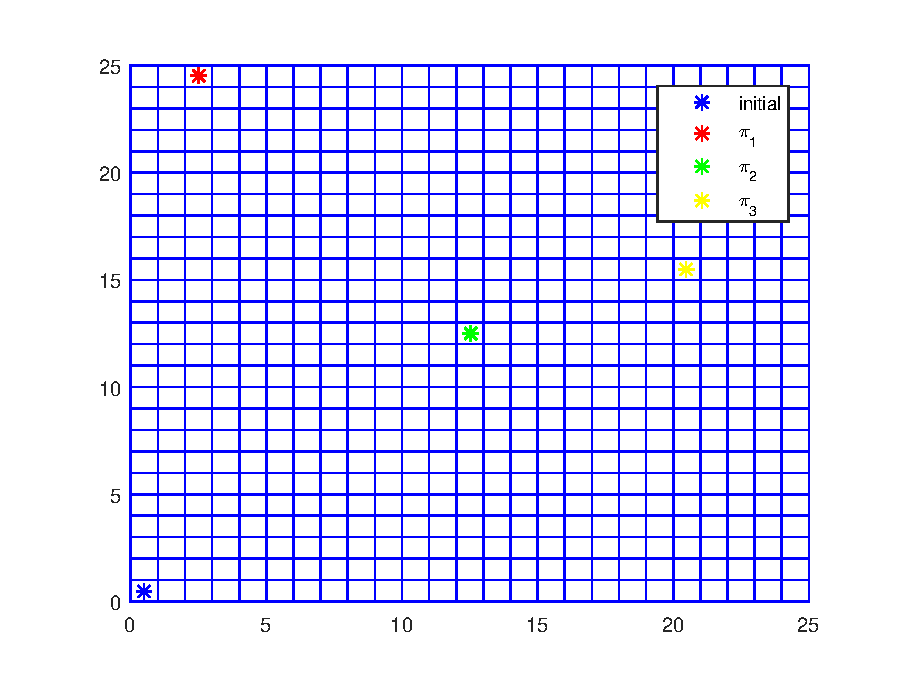
\includegraphics[scale=1]{workspace.eps}
\label{fig:workspace}
\end{figure}


When we use our algorithm on a coverage formula, we may not get the optimal path. We will however get an accepting path, and we now show that this path corresponds to the one generated by the nearest neighbour approach to the travelling salesperson problem. We also provide a provide a bound on the distance of our path based on the worst case ratio of the nearest neighbour tour to the optimal tour given by Rosendrantz, Stearns, and Lewis \cite{rosenkrantz74}. The travelling salesperson problem is stated in layman's terms as finding the shortest path for a salesperson to take such that he passes through a given set of cities and then returns back home at the end. More formally, it can be stated as finding the minimum Hamiltonian circuit with the lowest sum of distances between the nodes (cities). This problem has been studied extensively and "give quote about importance". This problem is NP-hard, and thus many algorithms and heuristics exist for finding an approximate solution. One very simple algorithm to do this is called the nearest neighbour algorithm. It says from the starting city, pick the closest city to be the next stop. From there, pick the next closest city not including the starting city, and so on. If there is a tie in the next closest neighbour, we assume that the next node can be decided arbitrarily. This is exactly what our algorithm does in this situation, the first Dijkstra search finds the closest node, and the we start another search. 

To formulate our problem as a travelling salesman problem we use the idea of a dummy node from Lenstra and Rinnooy Kan's computer wiring example in \cite{lenstra75}. In their example, they are designing a computer interface at the Institute for Nuclear Physical Research in Amsterdam. An interface is made up of several modules, with multiple pins on each module. A given subset of pins has to be interconnnected by wires, and at most two wires can be connected to any pin. For obvious regions, it is desirable to minimize the amount of wire used. They show that this is actually a travelling salesperson problem in disguise. The only difference between this problem and a travelling salesman problem is that in the travelling salesman problem, the salesman must return home at the end. This is not true in this problem. It is also not true in our problem, we only need to pass through $\pi_1$, $\pi_2$ and $\pi_3$, there is no need to return to the starting state after we do this. To formulate this seemingly unrelated problem into a travelling salesperson problem, they set $P$ to be the set of pins to be interconnected, $c_{ij}$ to be the distance between pin $i$ and pin $j$. They then introduce a dummy node $*$ that is a distance 0 from all the other nodes i.e.\ $c_{i*} = c_{*i} = 0$ for all i. Then the corresponding problem is solving the travelling salesperson problem on the set of nodes $N=P \cup \{*\}$. 

For our problem, we set $c_{ij}=d(\pi_i , \pi_j)$, for $i,j=0,1,2,3$ where where the initial state is from now on known as $\pi_0$, to be the shortest path our robot can take from $\pi_i$ to $\pi_j$, insuring that the triangle inequality is satisfied for all $i$ and $j$. We must preserve the the triangle inequality for a proof of a worst case scenario bound we will provide later on. We use this same idea as above of adding a dummy node, however to preserve the triangle inequality we cannot have the dummy node be distance 0 from the other nodes. Indeed, if $c_{i*} = c_{*i} = 0 $ the triangle inequality would be violated because $c_{i*} + c_{*j} = 0 \geq c_{ij}$ which would make the cost from getting to any point 0, thus rendering the problem extremely trivial. 

We can represent the relationship between the regions in our graph with the following \textit{complete} subgraph, shown in figure. A complete graph is an undirected graph in which every pair of vertices is connected by an edge. 
\begin{figure}
\centering
\begin{tikzpicture}[-,>=stealth',shorten >=1pt,auto,node distance=4cm,
                    semithick]
  \tikzstyle{every state}=[fill=red,draw=black,text=black]

  \node[state] (A)                    {Initial};
  \node[state] (B)                    [right of=A]{$\pi_1$};
  \node[state] (C)                    [below of=A]{$\pi_2$};
  \node[state]         (D) [right of=C] {$\pi_3$};

  \path (A) edge              node {$26$} (B)
  		(A) edge 			 node {$24$} (C)
  		(A) edge              node {$35$} (D)
  		(B) edge 				node {$22$} (C)
  		(B) edge              node {$27$} (D)
  		(C) edge				node {$11$} (D);
\end{tikzpicture}
\caption{Example 1: $BA$}
\label{fig:completeGraph}
\end{figure}

For the distances, we use the so called \textit{Manhatten distance}, i.e.\ $d((x_1,y_1),(x_2,y_2)) = |x_1 - x_2| +| y_1 - y_2|$ because our robot can only move horizontally and vertically, not diagonally. Given the weights between the vertices, we easily see that the path that our algorithm, and the nearest neighbour, will take is shown in figure \ref{fig:pathOnComplete}. The cost of this path is 62.

\begin{figure}
\centering
\begin{tikzpicture}[-,>=stealth',shorten >=1pt,auto,node distance=4cm,
                    semithick]
  \tikzstyle{every state}=[fill=red,draw=black,text=black]

  \node[state] (A)                    {I$\pi_0$};
  \node[state] (B)                    [right of=A]{$\pi_1$};
  \node[state] (C)                    [below of=A]{$\pi_2$};
  \node[state]         (D) [right of=C] {$\pi_3$};

  \path (A) edge 			 node {$24$} (C)
  		(B) edge              node {$27$} (D)
  		(C) edge				node {$11$} (D);
\end{tikzpicture}
\caption{Example 1: $BA$}
\label{fig:pathOnComplete}
\end{figure}

This is not the optimal path though, which is shown in figure \ref{fig:optcompleteGraph} and has a cost of 59.

\begin{figure}
\centering
\begin{tikzpicture}[-,>=stealth',shorten >=1pt,auto,node distance=4cm,
                    semithick]
  \tikzstyle{every state}=[fill=red,draw=black,text=black]

  \node[state] (A)                    {Initial};
  \node[state] (B)                    [right of=A]{$\pi_1$};
  \node[state] (C)                    [below of=A]{$\pi_2$};
  \node[state]         (D) [right of=C] {$\pi_3$};

  \path (A) edge              node {$26$} (B)
  		%(A) edge 			 node {$24$} (C)
  		%(A) edge              node {$35$} (D)
  		(B) edge 				node {$22$} (C)
  		%(B) edge              node {$27$} (D)
  		(C) edge				node {$11$} (D);
\end{tikzpicture}
\caption{Example 1: $BA$}
\label{fig:optcompleteGraph}
\end{figure}


Because we have to make sure that the dummy node does not change the order that our algorithm and the nearest neighbour algorithm takes we have to set the distance the dummy node is away from every other node to be $max_{i,j} c_{ij} $ where $c_{ij}$ is the distance between the nodes in the complete subgraph in figure \ref{fig:completeGraph}. In our case, this is 35, the path between $\pi_0$ and $\pi_3$. This insures that the path taken is the same as the accepted neighbour because the dummy node will be the last node to be visited. This is because in the nearest neighbour algorithm, ties are broken arbitrarily. Thus, the only time where it is a possibility that the nearest neighbour algorithm goes to the dummy node i.e.\ when the next nodes are $\max_{i,j} c_{ij}$ from the current node is when and if we are faced with the only choice being take the maximum path $\max_{i,j} c_{i,j}$ to $\pi_j$ or to go to the dummy node, and we can choose to go to $\pi_j$ because the ties can be broken arbitrarily. In any other case, the nearest neighbour path will choose a to go to a node where the cost is $c_{i',j'} < c_{i,j}$. 

We show the new subgraph in figure \ref{fig:completeDummy}

\begin{figure}
\centering
\begin{tikzpicture}[-,>=stealth',shorten >=1pt,auto,node distance=4cm,
                    semithick]
  \tikzstyle{every state}=[fill=red,draw=black,text=black]

  \node[state] (A)                    {$\pi_0$};
  \node[state] (B)                    [right of=A]{$\pi_1$};
  \node[state] (C)                    [below of=A]{$\pi_2$};
  \node[state]         (D) [right of=C] {$\pi_3$};
  \node[state] (E)			[right of = D] {$*$}; 

  \path (A) edge              node {$26$} (B)
  		(A) edge 			 node {$24$} (C)
  		(A) edge              node {$35$} (D)
  		(B) edge 				node {$22$} (C)
  		(B) edge              node {$27$} (D)
  		(C) edge				node {$11$} (D)
  		(E) edge 				node {$35$} (D)
  		(E) edge 				[bend left] node {$35$} (C)
  		(E) edge 				node {$35$} (B)
  		(E) edge 				node {$35$} (A);
\end{tikzpicture}
\caption{Example 1: $BA$}
\label{fig:completeDummy}
\end{figure}

The path that the nearest neighbour algorithm takes in this situation, the complete Hamiltonian circuit, is given in figure \ref{fig:NearNeigDummy}, which gives a total cost of 132.

\begin{figure}
\centering
\begin{tikzpicture}[-,>=stealth',shorten >=1pt,auto,node distance=4cm,
                    semithick]
  \tikzstyle{every state}=[fill=red,draw=black,text=black]

  \node[state] (A)                    {$\pi_0$};
  \node[state] (B)                    [right of=A]{$\pi_1$};
  \node[state] (C)                    [below of=A]{$\pi_2$};
  \node[state]         (D) [right of=C] {$\pi_3$};
  \node[state] (E)			[right of = D] {$*$}; 

  \path (A) edge 			 node {$24$} (C)
  		%(A) edge              node {$35$} (D)
  		%(B) edge 				node {$22$} (C)
  		(B) edge              node {$27$} (D)
  		(C) edge				node {$11$} (D)
  		%(E) edge 				node {$35$} (D)
  		%(E) edge 				[bend left] node {$35$} (C)
  		(E) edge 				node {$35$} (B)
  		(E) edge 				node {$35$} (A);
\end{tikzpicture}
\caption{Example 1: $BA$}
\label{fig:NearNeigDummy}
\end{figure}

We node however that this is not the optimal solution. This optimal solution is shown in 
figure \ref{fig:optDummy} and has a cost of 129.

\begin{figure}
\centering
\begin{tikzpicture}[-,>=stealth',shorten >=1pt,auto,node distance=4cm,
                    semithick]
  \tikzstyle{every state}=[fill=red,draw=black,text=black]

  \node[state] (A)                    {$\pi_0$};
  \node[state] (B)                    [right of=A]{$\pi_1$};
  \node[state] (C)                    [below of=A]{$\pi_2$};
  \node[state]         (D) [right of=C] {$\pi_3$};
  \node[state] (E)			[right of = D] {$*$}; 

  \path (A) edge			node {$26$} (B)
  		%(A) edge 			 node {$24$} (C)
  		%(A) edge              node {$35$} (D)
  		(B) edge 				node {$22$} (C)
  		%(B) edge              node {$27$} (D)
  		(C) edge				node {$11$} (D)
  		(E) edge 				node {$35$} (D)
  		%(E) edge 				[bend left] node {$35$} (C)
  		%(E) edge 				node {$35$} (B)
  		(E) edge 				node {$35$} (A);
\end{tikzpicture}
\caption{Example 1: $BA$}
\label{fig:optDummy}
\end{figure}



It has been shown that for an n-node travelling salesperson problem which satisfies the triangle inequality i.e.\ $d(i,j) = d(j,k) \geq d(i,k)$ for all $i,j,$ and $k$ where $d(i,j)$ is the nonnegative distance between nodes $i$ and $j$, 
\begin{align*}
\text{NEARNEIBR} \leq (\frac{1}{2} \lceil \log(n) \rceil + \frac{1}{2})\text{OPTIMAL}
\end{align*}
where NEARNEIBR is the cost of the path generated by the nearest neighbour algorithm and OPTIMAL is the cost of the optimal path. 

Our values do indeed satisfy this inequality
\begin{align*}
\text{NEARNEIBR} &\leq (\frac{1}{2} \lceil \log(n) \rceil + \frac{1}{2})\text{OPTIMAL}
132 &\leq (\frac{1}{2} \lceil \log(5) \rceil + \frac{1}{2})129
132 &\leq (2)129
132 \leq 258 
\end{align*}
We also see that it is very conservative worst case bound and we will likely do much better.

We provide a proof of
\begin{align}
\dfrac{\text{NEARNEIBR}}{\text{OPTIMAL}} \leq \frac{1}{2} \lceil \log(n) \rceil + \frac{1}{2}
\end{align}
which can be found in \cite{rosenkrantz74}. 
Proof:
We begin by proving 
\begin{align}
\text{OPTIMAL} \geq 2 \sum^{\min(2k,n)}_{i=k+1} l_i \label{eq:showFirst}
\end{align}
for all $k$, $0\leq k \leq n$. 
Let $l_i$ be the length of the $i^{th}$ largest edge in the tour obtained by the nearest neighbour algorithm. For each $i$, $0 \leq i \leq n$, let $a_i$ be the node \textit{onto which} the $i^{th}$ largest edge is added to (that would be the edge with length $l_i$). Let $H$ be the complete subgraph defined on the set of nodes $\{a_i | 1 \leq i \leq min(2k,n)\}$.

Now, let $T$ be the tour in $H$ which visits the nodes of $H$ in the same order as these nodes are visited in an optimal tour of the original graph. Let LENGTH be the length of $T$. We have 
\begin{align}
\text{OPTIMAL $\geq$ LENGTH} \label{eq:optglen}
\end{align}
This is because the tour with cost OPTIMAL passes through all the nodes that the tour with cost LENGTH passes through, and more. Thus if H has an edge $(b,c)$, then the OPTIMAL tour will either have the edge $(b,c)$ or take a less direct route through some of its extra nodes. So the triangle inequality implies (\ref{eq:optglen}).  
   
Let $(a_i,a_j)$ be an edge of $T$. If the nearest neighbour method adds point $a_i$ before $a_j$, we have $d(a_i,a_j) \geq l_i$, where $d(a_i,a_j)$ is the distance between nodes $a_i$ and $a_j$. We also see that if $a_j$ is added first we have $d(a_i, a_j) \geq l_j$. This is because, say we added $a_i$ first, we know there is a point $l_i$ away from $a_i$ that the nearest neighbour method makes the path to. This can be $a_j$, because we know $a_j$ has not been added yet or another node. If it is another node $d(a_i, a_j) \geq l_i$ because the nearest neighbour finds the closest node that has not yet been visited, or $d(a_i, a_j) = l_i$ if $a_j$ is added next. 

Since one has to be added before the other, we have 
\begin{align}
d(a_i , a_j) \geq \min(l_i, l_j) \label{ex:oneBefore}
\end{align}

Summing (\ref{ex:oneBefore}) over the edges of $T$, we get
\begin{align}
\text{LENGTH} \geq \sum_{(a_i,a_j) \text{ in } T} \min(l_i,l_j)  \label{eq:lengmin}
\end{align}

If we let $\alpha_i$ be the number of edges $(a_i, a_j)$ in $T$ for which $l_i$ is selected as $\min(l_i, l_j)$ we obtain 

\begin{align}
\sum_{(a_i,a_j) \text{ in } T} \min(l_i, l_j) = \sum_{a_i \text{ in } H} a_i l_i  \label{ex:lowBound}
\end{align}

Because $a_i$ is the endpoint of two edges in $T$, $\alpha \leq 2$. 

Because $T$ has $\min(2k,n)$ edges (one for each node),

\begin{align}
\sum_{a_i \text{ in } H} \alpha_i = \min(2k,n) 
\end{align}

To get a lower bound on (\ref{ex:lowBound}) we assume that $\alpha_i = 2 $ for $k+1 \leq i \leq \min(2k,n)$ and is zero of $i \leq k$. Thus,

\begin{align}
\sum_{a_i \text{ in } H} a_i l_i \geq 2 \sum_{i=k+1}^{\min(2k,n)} l_i \label{eq:alg2}
\end{align}

Combining (\ref{eq:optglen}), (\ref{eq:lengmin}), (\ref{ex:lowBound}), and (\ref{eq:alg2}), we get

\begin{align*}
\text{OPTIMAL} \geq \text{LENGTH} \geq \sum_{(a_i,a_j) \text{ in } T} \min(l_i,l_j) = \sum_{a_i \text{ in } H} a_i l_i \geq 2 \sum_{i=k+1}^{\min(2k,n)} l_i
\end{align*}
thus proving (\ref{eq:showFirst}). 

We now sum (\ref{eq:showFirst}) for all values of $k$ for all values of $k$ equal to powers of two less than or equal to $n$ i.e. $k = 2^{j} \leq n$ for $j = 0, 1, \dots \lceil \log(n) \rceil - 1$. We then get

\begin{align*}
\sum_{j=0}^{\lceil \log(n) \rceil -1} \text{OPTIMAL} \geq \sum_{j=0}^{\lceil \log(n) \rceil - 1} ( 2 \cdot \sum_{i=2^j + 1}^{\min(2^{j+1,n})} l_i )
\end{align*}
We have
\begin{align*}
\sum_{j=0}^{\lceil \log(n) \rceil -1} \text{OPTIMAL} &\geq 2 \cdot \sum_{i=2}^2 l_i + 2 \cdot \sum_{i=3}^4 l_i + 2 \cdot \sum_{i=5}^8 + \sum_{j=3}^{\lceil log(n) \rceil - 1} (2 \cdot \sum_{i = 2^j+1}^{\min(2^{j+1},n)} l_i )\\
& \geq 2 l_2 + 2 l_3 + 2 l_4 \dots +2l_8 + \sum_{j=3}^{\lceil log(n) \rceil - 1} (2 \cdot \sum_{i = 2^j+1}^{\min(2^{j+1},n)} l_i)
\end{align*}

Therefore we can write

\begin{align}
\lceil \log(n) \rceil \cdot \text{OPTIMAL} \geq 2 \sum_{i = 2}^n l_i \label{eq:lognoptt}
\end{align}

Now OPTIMAL must be longer than twice any edge in the graph because it contains two paths between any given pair of points and these paths are , by the triangle  inequality, longer than the distance of the edge connecting the points directly, i.e.\ OPTIMAL $\geq 2 l_i$ for $i = 1,2,\dots, n$. Specifically,
\begin{align}
\text{OPTIMAL} \geq 2 \l_1 \label{eq:optgl1}
\end{align}

Summing (\ref{eq:lognoptt}) and (\ref{eq:optgl1}) we get 
\begin{align*}
(\log(n)+1) \cdot \text{OPTIMAL} \geq 2 \sum_{i=1}^n l_i
\end{align*}
By definition, $\sum_{i=1}^n l_i = \text{NEARNEIBR}$, thus we have 
\begin{align*}
\text{NEARNEIBR} \leq (\frac{1}{2} \lceil \log(n) \rceil + \frac{1}{2}) \text{OPTIMAL}
\end{align*}
\qed 

We have thus shown that when formulating and solving our problem as a travelling salesman problem with a dummy node, we get the same solution as the nearest neighbour search algorithm. This search algorithm then has a bound on the worst case cost of the resulting solution in teams of the cost of the optimal solution i.e.\ 
\begin{align*}
\text{NEARNEIBR} \leq (\frac{1}{2} \lceil \log(n) \rceil + \frac{1}{2}) \text{OPTIMAL}
\end{align*}

We now must remove the dummy node and provide a bound for the true cost that we will get from our search. 

NEARNEIBR and OPTIMAL as above are costs of Hamaltonian circuits. By definition every node in a Hamaltonian circuit is passed through exactly once. Therefore the dummy node will be passed through exactly once, and we have shown that it will be the last node passed through in the NEARNEIBR. In the NEARNEIBR path, because the dummy node is length $\max_{i,j} c_{i,j}$ it will never be the closest next node, unless we are given the choice to go from $\pi_i$ to $\pi_j$ for $i$ and $j$ being the maximum edge cost in the complete subgraph. In this case we can break the tie arbitrarily and choose to go to $\pi_j$ instead of the dummy node. Thus the path found by the nearest neighbour search will be the path found by our our algorithm, and then going to the dummy node for a cost of $\max_{i,j} c_{i,j}$, then from there going to the initial node to for a cost of $\max_{i,j} c_{i,j}$. Therefore the cost of our algorithm, denote ALGOR is 
\begin{align*}
\text{ALGOR = NEARNEIBR - } 2\max_{i,j} c_{i,j} 
\end{align*}

The path OPTIMAL, however is not guaranteed to have the dummy node be the last node visited. The cost of the path which is optimal and requires that the dummy node is the last node visited, is then greater than or equal to OPTIMAL. This is because of the freedom taken away by requiring the dummy node to be visited last, and less freedom in a minimization problem results in a larger value. Let ACCEPT be the cost of the accepted algorithm for path planning. ACCEPT $+ 2\max_{i,j} c_{i,j}$ is then equal to the cost of the optimal travelling salesman solution which requires that the dummy node is the last node visited. This is because we have already established that the accepted algorithm will find the optimal path. Therefore we have
\begin{align*}
\text{ACCEPT} + 2\max_{i,j} c_{i,j} \geq \text{OPTIMAL}
\end{align*}

Plugging into the travelling salesman bound, we get
\begin{align*}
\text{NEARNEIBR} &\leq (\frac{1}{2} \lceil \log(n) \rceil + \frac{1}{2}) \text{OPTIMAL} \\
\text{ALG} + 2\max_{i,j} c_{i,j} &\leq (\frac{1}{2} \lceil \log(n) \rceil + \frac{1}{2}) \text{OPTIMAL} \\
\text{ALG} + 2\max_{i,j} c_{i,j} &\leq (\frac{1}{2} \lceil \log(n) \rceil + \frac{1}{2}) (\text{ACCEPT} + 2 \max_{i,j} c_{i,j} \\ 
\end{align*} 

We can check with our previously calculated values for ALG and ACCEPT
\begin{align*}
\text{ALG} + 2\max_{i,j} c_{i,j} &\leq (\frac{1}{2} \lceil \log(n) \rceil + \frac{1}{2}) (\text{ACCEPT} + 2 \max_{i,j} c_{i,j} \\ 
62 + 2 (35) &\leq (\frac{1}{2} 3 + \frac{1}{2})(59+2(35)) \\
132 &\leq 258
\end{align*}
We can see that this is still a conservative bound, and emphasize that it is the worst case. Usually the algorithm will preform much better.


\subsection{Recurrence (Liveness)}
Recurrence is coverage over and over again, and can be expressed as $\square(\diamond \pi_1 \land \diamond \pi_2 \land \dots \land \diamond \pi_n)$. This example is interesting for two reasons: it is prone to B\"{u}chi automata that are not tight, and it an accepting path for it does cannot stay in one state (in contrast to the other formulas, in which all accepting states have self loops). We first look at the tightness.

To illustrate our point, we consider the formula $\square(\diamond \pi_1 \land \diamond \pi_2 \land \diamond \pi_3)$. The B\"{u}chi automaton corresponding to this formula, as calculated by \cite{gastin01} is 

\begin{figure}
\centering
\begin{tikzpicture}[->,>=stealth',shorten >=1pt,auto,node distance=2.8cm,
                    semithick]
  \tikzstyle{every state}=[fill=red,draw=black,text=black]

  \node[initial,state] (A)                    {$q_1$};
  \node[state] (B)                    [right of=A]{$q_2$};
  \node[state,accepting] (C)                    [right of=B]{$q_3$};

  \path (A) edge              node {$\pi_{1}$} (B)
  		(A) edge [loop above] node {$\neg \pi_1$} (A)
  		(B) edge [loop above] node {$\neg \pi_2$} (B)
  		(B) edge              node {$\pi_{2}$} (C)
  		(C) edge [bend left=45] node {$\neg \pi_1$} (A)
  		(C) edge  [bend left] node {$\pi_{1}$} (B);
%  		(D) edge [bend right] node {$\neg \pi_1$} (A)
 % 		(D) edge [bend left] node {$\pi_1$} (B);
\end{tikzpicture}
\caption{Example 1: $BA$}
\label{fig:gasBuchiRec}
\end{figure}
Note: The actual automaton generated has much more edges. For example, there is an edge from $q_4$ to $q_2$ which is labelled $\pi_1 \&\& \pi_2$. It is impossible for us to make this transition because $\pi_i$ for all $i$ is a region in our partition. This is because the requirements of our partition are chosen specially to guarantee that we are never in two regions at once. Thus they are excluded in the interest of the reader. In this automation, $d(q_1)=2$, $d(q_2)=1$, and $d(q_3)=0$. So, to get from $q_{init}' = \langle \pi_2, q_1 \rangle \in Q_0'$, we have to first get down to level 2. Given the B\"{u}chi automaton \ref{fig:gasBuchiRec} the only way to do this is to go to region $\pi_1$. Our algorithm does this, and then starts a new Dijkstra search. In this case the same statement holds for $\pi_2$. Therefore the optimal prefix is to concatenate the optimal paths down from each each level (first to $\pi_1$, etc). Our algorithm does a Dijkstra search at each level so it will return this path as the prefix. The accepted algorithm will also return this prefix. 

This path however is in general not truly optimal. It is because the B\"{u}chi automaton given in figure \ref{fig:gasBuchiRec} not a tight B\"{u}chi automaton \cite{schuppan05}. A B\"{u}chi automaton is tight if it accepts the shortest lasso (prefix and suffix). The loss of this optimality property is due to the fact that the algorithm in \cite{gastin01} simplifies the B\"{u}chi automaton which is usually a good thing because it leads to a lower computational complexity in most applications. We take a look at a different automaton corresponding to the formula $\square(\diamond \pi_1 \land \diamond \pi_2)$, shown in figure \ref{fig:otherBuchiRec}. 

\begin{figure*}
\centering
\begin{tikzpicture}[->,>=stealth',shorten >=1pt,auto,node distance=3.7cm,
                    semithick]
  \tikzstyle{every state}=[fill=red,draw=black,text=black]

  \node[initial,state] (A)                    {$q_1$};
  \node[state]         (B) [ right of=A] {$q_2$};  
  \node[state] 		   (C)  [below of=B]  {$\pi_3$};
  \node[state,accepting]       (D) [ right of=C] {$q_4$};

  \path (A) edge         node {$\pi_{1}$}   (B)
        (B) edge       node {$\pi_{2}$}     (D)
        (A) edge       node {$\pi_{2}$}  (C)
        (C) edge     node {$\pi_{1}$}       (D)
        (A) edge [loop above] node {$\neg \pi_1 \wedge \neg \pi_2$} (A)
        (B) edge [loop above] node {$\neg \pi_2$} (B)
        (C) edge [loop below] node {$\neg \pi_1$} (C)
        (D) edge [bend left] node {$\pi_2$} (C)
        (D) edge [bend left] node {$\pi_1$} (B)
        (D) edge node{$\neg \pi_1 \wedge \neg \pi_2$} (A);
\end{tikzpicture}
\caption{Product Automaton}
\label{fig:otherBuchiRec}
\end{figure*}

In this automaton, $d(q_1) = 2$, $d(q_2) = d(q_3) = 1$, and $d(q_4)= 0$. So, we are starting at the same level i.e. 2, however this time we have two choices about what to do to get down to level 2; we can go to $\pi_1$ or $\pi_2$. Being able to choose is good in the sense that we can now find the optimal path, and bad in the sense that the extra state in the $B\"{u}chi$ automaton increased the size of the product automaton by 33\% (hence increasing the time it takes to search the automaton). This very well illustrates the trade off between the search time and optimally/cost of the resulting run. We propose that this is a good way to think about our algorithm. There is a trade off that sometimes it will not find the optimal run, even if this is possible, though it will be faster. 

The second aspect of this problem that we wish to look at is fact that it does not have a trivial suffix. In the other examples we have looked at, the suffix of the calculated path (with our algorithm and the accepted algorithm) was a single state; that is, the formula could be satisfied by staying in one state indefinitely. In this example, $\pi_1,$ $\pi_2$, and $\pi_3$ must all be visited infinitely often, and thus these states must be in the suffix. 

The applicability of our algorithm to find the suffix has to be considered. For the total run, R, to be accepting, $\Inf(R) \cap \F$ must not be empty. We are specifically looking for runs of the form 
\begin{align*}
R &= \langle R_{pre}, R_{suf} \rangle = q_0 q_1 \dots q_f [q_f q_{f+1} \dots q_n]^\omega
\end{align*}     
where $q_f \in \F$. Thus when calculating to the suffix we must find the path back to the \textit{same} accepting state. We cannot not just look for any accepting state as we do in the prefix calculation. Our algorithm in general only looks for an accepting state, not a specific accepting state; however in certain circumstances it can find a specific accepting state. We illustrate this using the same examples above. 

$\square (\diamond \pi_3 \wedge \pi_5)$ 
We notice how in figure \ref{fig:gasBuchiRec} there is only one arrow to the accepting state, labelled $\pi_5$. This implies that the only way to get down to level 0 is to go to $\pi_5$, and thus go to the accepting state $\langle \pi_5, q_3 \rangle$. There is no self loop on $q_3$, so we leave $q_3$ immediately. This implies that the only reachable accepting state is $\langle \pi_5, q_3 \rangle$. So because there is only one accepting state, our algorithm will find this state again, and thus is appropriate for finding the suffix. 

In \ref{fig:otherBuchiRec} on the other hand, there are two arrows going to the accepting state and there is no self loop. This implies that there are two reachable accepting states i.e.\ $\langle \pi_3, q_4 \rangle$ and $\langle \pi_5, q_4 \rangle$. This poses a problem to our algorithm that is only guaranteed to reach an accepting state. We thus propose using Dijkstra's search algorithm to find the path from the accepting node back to itself.   

